% Options for packages loaded elsewhere
% Options for packages loaded elsewhere
\PassOptionsToPackage{unicode}{hyperref}
\PassOptionsToPackage{hyphens}{url}
%
\documentclass[
  ignorenonframetext,
  aspectratio=169,
  russian,
]{beamer}
\newif\ifbibliography
\usepackage{pgfpages}
\setbeamertemplate{caption}[numbered]
\setbeamertemplate{caption label separator}{: }
\setbeamercolor{caption name}{fg=normal text.fg}
\beamertemplatenavigationsymbolsempty
% Prevent slide breaks in the middle of a paragraph
\widowpenalties 1 10000
\raggedbottom
\AtBeginPart{
  \frame{\partpage}
}
\AtBeginSection{
  \ifbibliography
  \else
    \frame{\sectionpage}
  \fi
}
\AtBeginSubsection{
  \frame{\subsectionpage}
}
\usepackage{iftex}
\ifPDFTeX
  \usepackage[T1]{fontenc}
  \usepackage[utf8]{inputenc}
  \usepackage{textcomp} % provide euro and other symbols
\else % if luatex or xetex
  \usepackage{unicode-math} % this also loads fontspec
  \defaultfontfeatures{Scale=MatchLowercase}
  \defaultfontfeatures[\rmfamily]{Ligatures=TeX,Scale=1}
\fi
\usepackage{lmodern}

\usetheme[progressbar=frametitle,sectionpage=progressbar,numbering=fraction]{default}
\ifPDFTeX\else
  % xetex/luatex font selection
\fi
% Use upquote if available, for straight quotes in verbatim environments
\IfFileExists{upquote.sty}{\usepackage{upquote}}{}
\IfFileExists{microtype.sty}{% use microtype if available
  \usepackage[]{microtype}
  \UseMicrotypeSet[protrusion]{basicmath} % disable protrusion for tt fonts
}{}
\makeatletter
\@ifundefined{KOMAClassName}{% if non-KOMA class
  \IfFileExists{parskip.sty}{%
    \usepackage{parskip}
  }{% else
    \setlength{\parindent}{0pt}
    \setlength{\parskip}{6pt plus 2pt minus 1pt}}
}{% if KOMA class
  \KOMAoptions{parskip=half}}
\makeatother


\usepackage{longtable,booktabs,array}
\usepackage{calc} % for calculating minipage widths
\usepackage{caption}
% Make caption package work with longtable
\makeatletter
\def\fnum@table{\tablename~\thetable}
\makeatother
\usepackage{graphicx}
\makeatletter
\newsavebox\pandoc@box
\newcommand*\pandocbounded[1]{% scales image to fit in text height/width
  \sbox\pandoc@box{#1}%
  \Gscale@div\@tempa{\textheight}{\dimexpr\ht\pandoc@box+\dp\pandoc@box\relax}%
  \Gscale@div\@tempb{\linewidth}{\wd\pandoc@box}%
  \ifdim\@tempb\p@<\@tempa\p@\let\@tempa\@tempb\fi% select the smaller of both
  \ifdim\@tempa\p@<\p@\scalebox{\@tempa}{\usebox\pandoc@box}%
  \else\usebox{\pandoc@box}%
  \fi%
}
% Set default figure placement to htbp
\def\fps@figure{htbp}
\makeatother



\ifLuaTeX
\usepackage[bidi=basic,provide=*]{babel}
\else
\usepackage[bidi=default,provide=*]{babel}
\fi
% get rid of language-specific shorthands (see #6817):
\let\LanguageShortHands\languageshorthands
\def\languageshorthands#1{}


\setlength{\emergencystretch}{3em} % prevent overfull lines

\providecommand{\tightlist}{%
  \setlength{\itemsep}{0pt}\setlength{\parskip}{0pt}}



 


\makeatletter
\@ifpackageloaded{caption}{}{\usepackage{caption}}
\AtBeginDocument{%
\ifdefined\contentsname
  \renewcommand*\contentsname{Содержание}
\else
  \newcommand\contentsname{Содержание}
\fi
\ifdefined\listfigurename
  \renewcommand*\listfigurename{Список иллюстраций}
\else
  \newcommand\listfigurename{Список иллюстраций}
\fi
\ifdefined\listtablename
  \renewcommand*\listtablename{Список таблиц}
\else
  \newcommand\listtablename{Список таблиц}
\fi
\ifdefined\figurename
  \renewcommand*\figurename{Рисунок}
\else
  \newcommand\figurename{Рисунок}
\fi
\ifdefined\tablename
  \renewcommand*\tablename{Таблица}
\else
  \newcommand\tablename{Таблица}
\fi
}
\@ifpackageloaded{float}{}{\usepackage{float}}
\floatstyle{ruled}
\@ifundefined{c@chapter}{\newfloat{codelisting}{h}{lop}}{\newfloat{codelisting}{h}{lop}[chapter]}
\floatname{codelisting}{Список}
\newcommand*\listoflistings{\listof{codelisting}{Листинги}}
\makeatother
\makeatletter
\makeatother
\makeatletter
\@ifpackageloaded{caption}{}{\usepackage{caption}}
\@ifpackageloaded{subcaption}{}{\usepackage{subcaption}}
\makeatother

\usepackage{bookmark}
\IfFileExists{xurl.sty}{\usepackage{xurl}}{} % add URL line breaks if available
\urlstyle{same}
\hypersetup{
  pdftitle={Лабораторная работа №1},
  pdfauthor={Чекмарев Александр Дмитриевич \textbar{} Группа НПИбд-03-24},
  pdflang={ru-RU},
  hidelinks,
  pdfcreator={LaTeX via pandoc}}


\title{Лабораторная работа №1}
\subtitle{Установка и конфигурация операционной системы на виртуальную
машину}
\author{Чекмарев Александр Дмитриевич \textbar{} Группа НПИбд-03-24}
\date{2025-06-09}

\begin{document}
\frame{\titlepage}

\renewcommand*\contentsname{Содержание}
\begin{frame}[allowframebreaks]
  \frametitle{Содержание}
  \setcounter{tocdepth}{2}
  \tableofcontents
\end{frame}
\setcounter{tocdepth}{2}
\tableofcontents
}

\section{1. Информация}\label{ux438ux43dux444ux43eux440ux43cux430ux446ux438ux44f}

\begin{frame}{1.1 Докладчик}
\phantomsection\label{ux434ux43eux43aux43bux430ux434ux447ux438ux43a}
\begin{columns}[c]
\begin{column}{0.7\linewidth}
\begin{itemize}
\tightlist
\item
  Чекмарев Александр Дмитриевич
\item
  Группа НПИбд-03-24
\item
  Российский университет дружбы народов им. П. Лумумбы
\end{itemize}
\end{column}

\begin{column}{0.3\linewidth}
\end{column}
\end{columns}
\end{frame}

\section{2. Вводная
часть}\label{ux432ux432ux43eux434ux43dux430ux44f-ux447ux430ux441ux442ux44c}

\begin{frame}{2.1 Объект и предмет исследования}
\phantomsection\label{ux43eux431ux44aux435ux43aux442-ux438-ux43fux440ux435ux434ux43cux435ux442-ux438ux441ux441ux43bux435ux434ux43eux432ux430ux43dux438ux44f}
\begin{itemize}
\tightlist
\item
  Установка ОС Linux Rocky на VirtualBox
\end{itemize}
\end{frame}

\begin{frame}{2.2 Цель работы}
\phantomsection\label{ux446ux435ux43bux44c-ux440ux430ux431ux43eux442ux44b}
\begin{itemize}
\tightlist
\item
  Целью данной работы является приобретение практических навыков
  установки операционной системы на виртуальную машину, настройки
  минимально необходимых для дальнейшей работы сервисов.
\end{itemize}
\end{frame}

\section{3. Ход лаборатороной
работы}\label{ux445ux43eux434-ux43bux430ux431ux43eux440ux430ux442ux43eux440ux43eux43dux43eux439-ux440ux430ux431ux43eux442ux44b}

\begin{frame}{3.1 Скачивание дистрибутива Rocky v10}
\phantomsection\label{ux441ux43aux430ux447ux438ux432ux430ux43dux438ux435-ux434ux438ux441ux442ux440ux438ux431ux443ux442ux438ux432ux430-rocky-v10}
\begin{itemize}
\tightlist
\item
  Скачиваем iso-образ Rocky актульной версии
\end{itemize}

\begin{figure}

{\centering 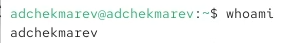
\includegraphics[width=0.7\linewidth,height=\textheight,keepaspectratio]{image/Screenshot_1.png}

}

\caption{Сайт: https://rockylinux.org/ru-RU/download}

\end{figure}%
\end{frame}

\begin{frame}{3.2 Настройки в VirtualBox для Rocky}
\phantomsection\label{ux43dux430ux441ux442ux440ux43eux439ux43aux438-ux432-virtualbox-ux434ux43bux44f-rocky}
\begin{itemize}
\tightlist
\item
  Выбираем iso образ, название, место
\item
  Выделяем ОЗУ
\item
  Выделяем 40 гб
\end{itemize}

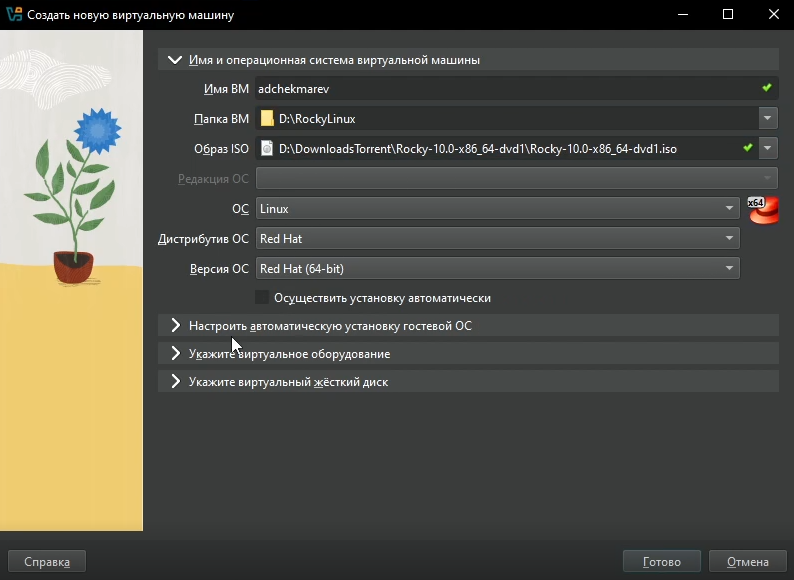
\includegraphics[width=0.35\linewidth,height=\textheight,keepaspectratio]{image/Рис 1.1.png}
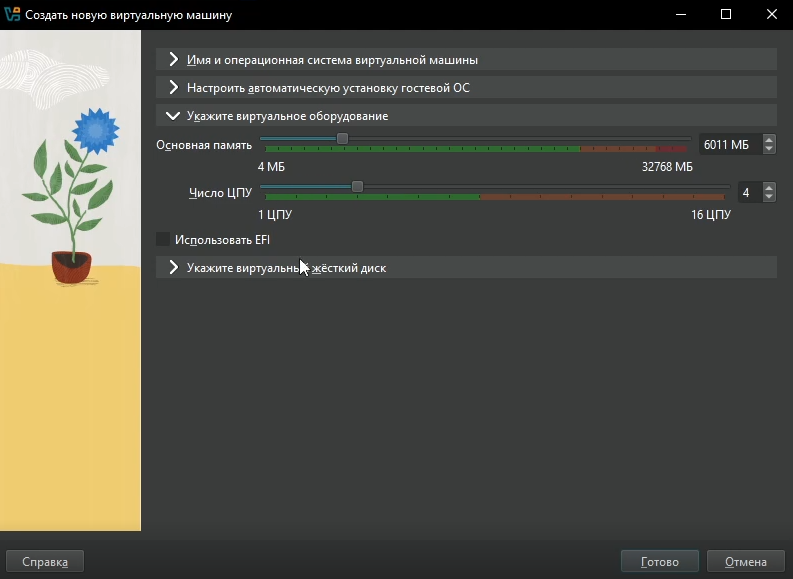
\includegraphics[width=0.35\linewidth,height=\textheight,keepaspectratio]{image/Рис 1.2.png}

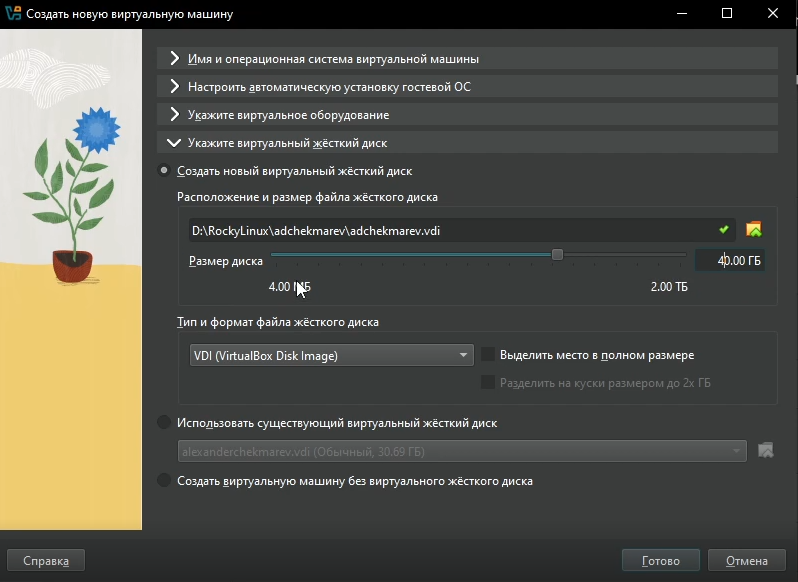
\includegraphics[width=0.35\linewidth,height=\textheight,keepaspectratio]{image/Рис 1.3.png}
\end{frame}

\begin{frame}{3.3 Настройки перед установкой (1)}
\phantomsection\label{ux43dux430ux441ux442ux440ux43eux439ux43aux438-ux43fux435ux440ux435ux434-ux443ux441ux442ux430ux43dux43eux432ux43aux43eux439-1}
\begin{itemize}
\tightlist
\item
  Выбираем нужный нам язык, жесткий диск и включаем root права для
  пользователя
\end{itemize}

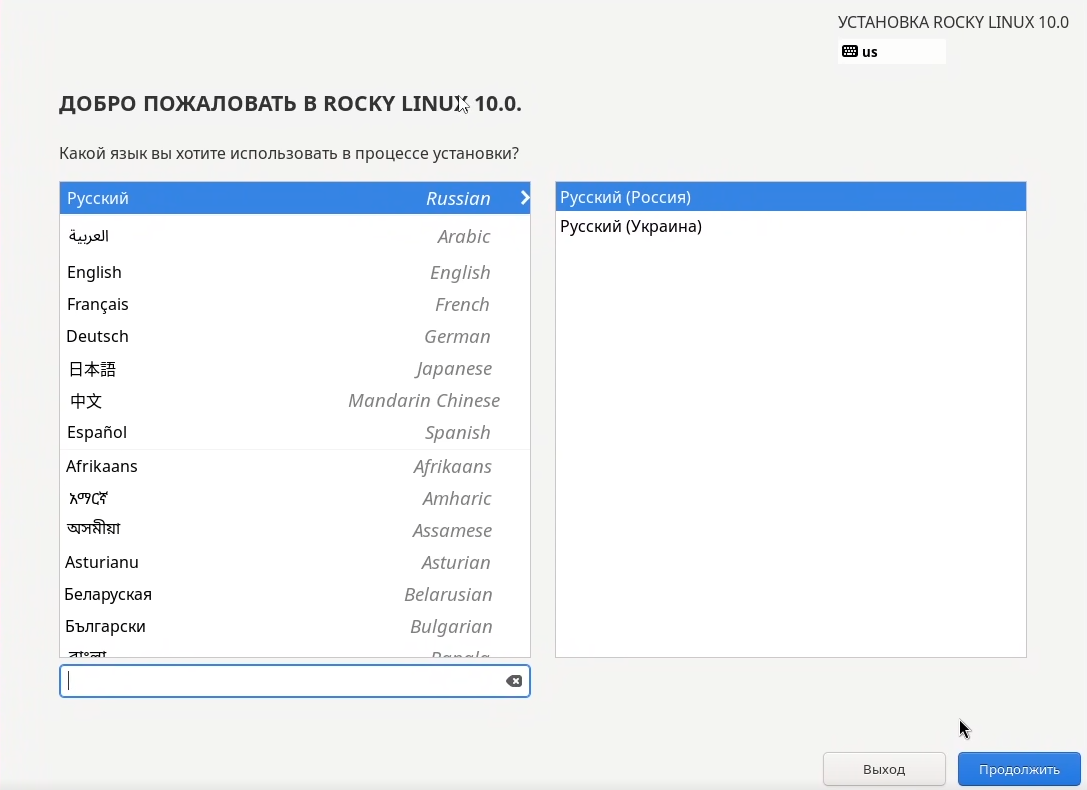
\includegraphics[width=0.35\linewidth,height=\textheight,keepaspectratio]{image/Рис 1.5.png}
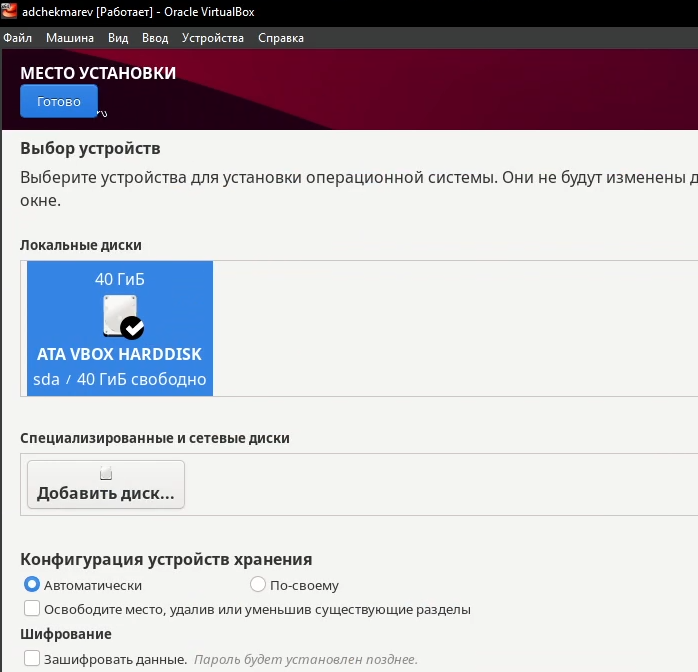
\includegraphics[width=0.35\linewidth,height=\textheight,keepaspectratio]{image/Рис 1.8.png}

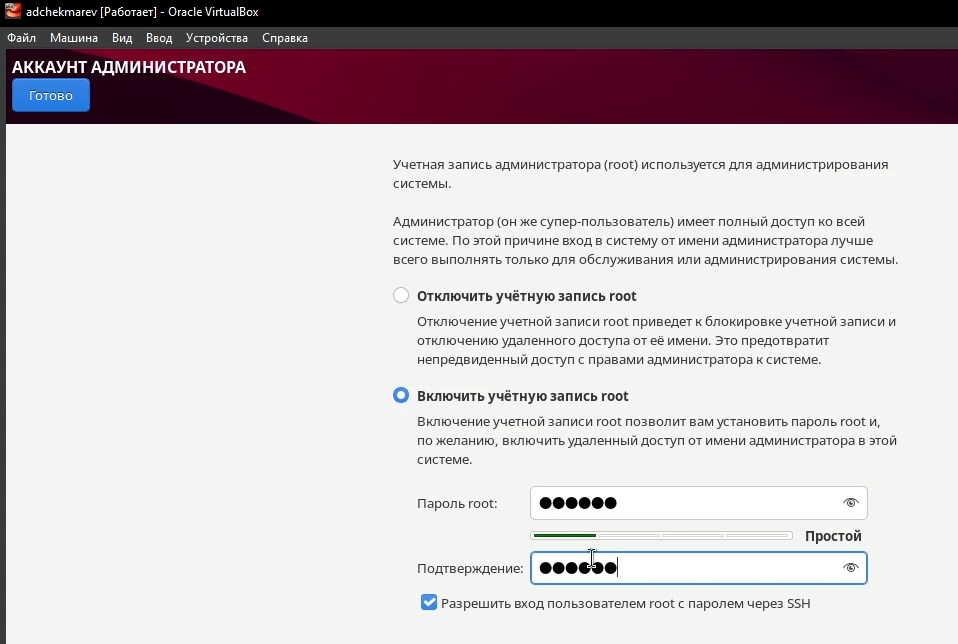
\includegraphics[width=0.35\linewidth,height=\textheight,keepaspectratio]{image/Рис 1.10.png}
\end{frame}

\begin{frame}{3.4 Настройки перед установкой (2)}
\phantomsection\label{ux43dux430ux441ux442ux440ux43eux439ux43aux438-ux43fux435ux440ux435ux434-ux443ux441ux442ux430ux43dux43eux432ux43aux43eux439-2}
\begin{itemize}
\tightlist
\item
  Выбираем нужные программы, отключаем KDUMP и меняем имя узла
\end{itemize}
\end{frame}

\begin{frame}{3.5 Настройка аккаунта пользователя и установка}
\phantomsection\label{ux43dux430ux441ux442ux440ux43eux439ux43aux430-ux430ux43aux43aux430ux443ux43dux442ux430-ux43fux43eux43bux44cux437ux43eux432ux430ux442ux435ux43bux44f-ux438-ux443ux441ux442ux430ux43dux43eux432ux43aux430}
\begin{itemize}
\tightlist
\item
  Создаем пользователя и приступаем к установке
\end{itemize}

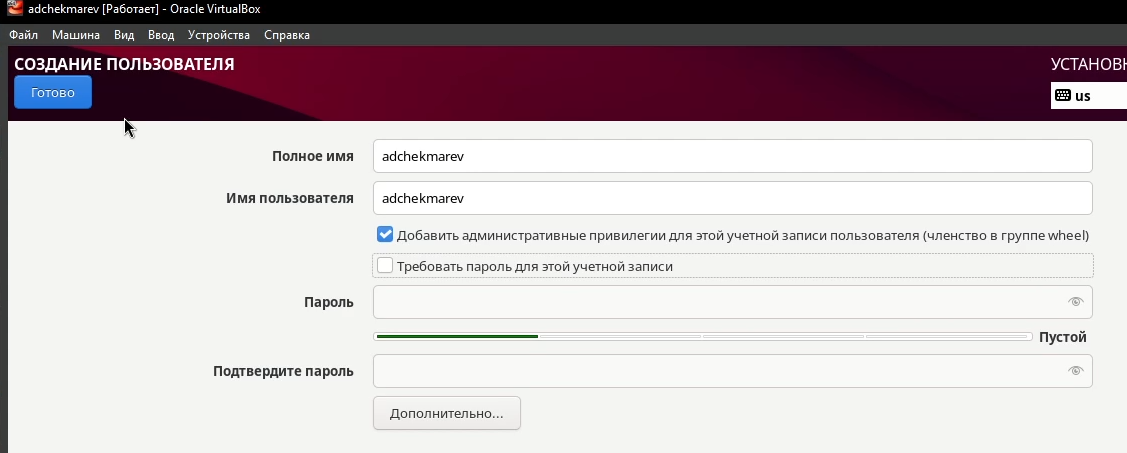
\includegraphics[width=0.4\linewidth,height=\textheight,keepaspectratio]{image/Рис 1.11.png}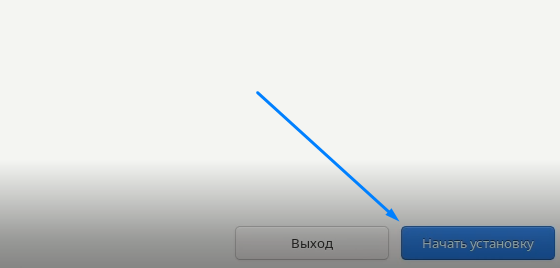
\includegraphics[width=0.4\linewidth,height=\textheight,keepaspectratio]{image/Screenshot_3.png}
\end{frame}

\begin{frame}{3.6 Подключение образа диска дополнений гостевой OC.}
\phantomsection\label{ux43fux43eux434ux43aux43bux44eux447ux435ux43dux438ux435-ux43eux431ux440ux430ux437ux430-ux434ux438ux441ux43aux430-ux434ux43eux43fux43eux43bux43dux435ux43dux438ux439-ux433ux43eux441ux442ux435ux432ux43eux439-oc.}
\begin{itemize}
\tightlist
\item
  Воспользуемся консольными командами для подключения образа диска
  дополнений гостевой OC.
\end{itemize}

\pandocbounded{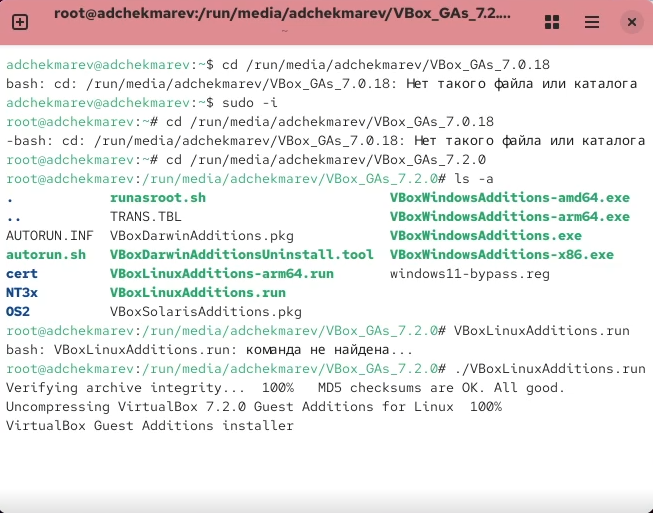
\includegraphics[keepaspectratio]{image/Рис 1.12.png}}

\begin{itemize}
\tightlist
\item
  После загрузки перезагрузим операцинную систему на виртуальной машине.
  На этом все готово
\end{itemize}
\end{frame}

\begin{frame}{3.7 Вывод:}
\phantomsection\label{ux432ux44bux432ux43eux434}
В процессе работы была установлена и настроена ОС Rocky Linux в среде
VirtualBox. Были получены навыки создания и конфигурации виртуальной
машины, работы с пользователями.
\end{frame}




\end{document}
